\documentclass{article}

\usepackage[final,nonatbib]{nips_2016}

\usepackage{url}
\usepackage{amsmath}
\usepackage{booktabs}
\usepackage{hyperref}
\usepackage{amsfonts}
\usepackage{nicefrac}
\usepackage{microtype}
\usepackage[T1]{fontenc}
\usepackage[utf8]{inputenc}
\usepackage[pdftex]{graphicx}
\usepackage[caption=false,font=footnotesize]{subfig}

\graphicspath{{./Images/}}
\DeclareGraphicsExtensions{.pdf,.jpeg,.png}

\title{Data-efficient Motor-skills Learning in Latent Spaces for Robotic Clothing Assistance}

\author{
  Nishanth Koganti$^{1,2}$, Tomoya Tamei$^{1}$, Kazushi Ikeda$^{1}$, Tomohiro Shibata$^{2}$\\
  $^1$ Nara Institute of Science and Technology, Japan~~~$^2$ Kyushu Institute of Technology, Japan\\
  \texttt{\{nishanth-k,tomo-tam,kazushi\}@is.naist.jp, tom@brain.kyutech.ac.jp} \\
}

\begin{document}

\maketitle

\begin{abstract}
Robotic implementation of clothing assistance can greatly improve the quality-of-life for the elderly and disabled. This is still considered an open problem as it involves close interaction of the robot with non-rigid clothing articles and the assisted person with varying posture. In this study, we propose a data-efficient representation to encode task specific motor-skills of the robot using Bayesian nonparametric latent manifold learning. We implement our framework in a practical setting with a dual-arm robot performing clothing tasks. We demonstrate that performing motor-skills learning in such task specific latent spaces outperforms learning in the high-dimensional joint configuration space of the robot. Furthermore, our framework can also be used as a tool for learning from demonstration to impart novel skills to the robot.
\end{abstract}

\section{Introduction}
\label{section:introduction}

Clothing assistance is a basic and important assistance activity in the daily life of the elderly and disabled people. However, robotic clothing assistance is still considered an open problem by most robotics researchers. Design of a robust framework involves reliable cloth state\ estimation in real-time and a motor skills learning framework that can detect and adapt to various failure scenarios. Existing studies do not explicitly handle these challenges and perform point-to-point motion planning in an offline manner for clothing assistance~\cite{yamazaki},\cite{gao}. An alternate approach is to formulate robotic clothing assistance as a reinforcement learning problem wherein the robot learns to recover from failure scenarios and adapt to new settings from experience.

Tamei \emph{et al.}~\cite{tamei} have proposed a reinforcement learning (RL) framework for clothing assistance with a dual-arm robot as the agent and a mannequin as the subject. The clothing task was to cloth the mannequin with a T-shirt which is initially on the mannequin's hands. The framework was formulated using low dimensional representations for the state and policy. The state was represented using topology coordinates which captured the relationship between the human and cloth extremities. The dual-arm robot's trajectory was parametrized using via-points which were obtained using a minimum jerk criterion. The policy was initialized using kinesthetic demonstration for a particular posture and the framework could successfully learn a policy for an unseen posture.

A limitation in the above framework is that policy search is performed in the kinematic space which is considerably high dimensional for a 7 degree of freedom (DOF) dual-arm robot. For tractable learning time, policy update was done using finite difference policy gradient applied to a single via-point of a single joint in each robot arm. This severely constrained the generalization capability to very different environmental settings such as major changes in the subject's posture or using different clothing article. To address this problem, we consider an alternate representation that is more flexible and suitable for robust learning of motor-skills. We propose the use of dimensionality reduction (DR) to learn a low-dimensional latent space that encodes clothing skills without losing any generalization capability.

In this study, we propose an efficient representation of motor skills that relies on the use of Bayesian Gaussian Process Latent Variable Model (BGPLVM)~\cite{bgplvm}. BGPLVM is capable of learning a data-efficient latent space for clothing tasks performed by a dual-arm robot. Representation of clothing skills in a low-dimensional space enables the use of expressive policy update rules for generalization to very different settings. We apply our proposed method to a clothing assistance setup as shown in Figure~\ref{figure:setup}. We demonstrate that the learned space generates robot trajectories that maintain task space constraints required for clothing tasks. We further present the design of a real-time controller from a BGPLVM latent space to a dual-arm robot. The experimental results indicate a promising policy representation with reinforcement learning that can be used for robotic clothing assistance.

The rest of the paper is structured as follows. Section~\ref{section:literature} provides an overview of related studies. The proposed framework is presented in Section~\ref{section:method}. Section~\ref{section:results} includes experimental results and Section~\ref{section:conclusion} concludes the paper with directions for future work.

\section{Related Work}
\label{section:literature}

\begin{figure}[t]
  \centering
  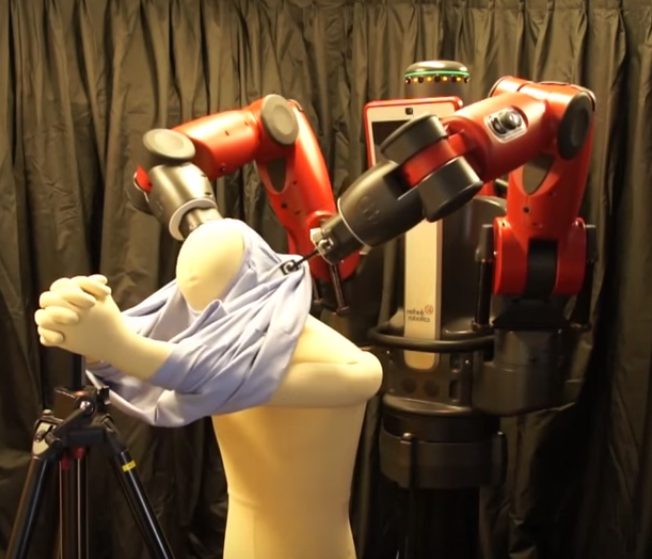
\includegraphics[width=0.45\textwidth, height=0.2\textheight]{setup.png}
  \caption{Clothing Assistance framework: Dual-arm robot clothing soft-mannequin with T-shirt.}
  \label{figure:setup}
\end{figure}

Motor skills learning for robots involves an agent interacting with a partially observable environment in continuous state and action spaces. Usually policy search reinforcement learning is applied wherein an optimal policy is learned by searching within the policy space. Reinforcement Learning usually suffer from the curse of dimensionality when applied to real-world situations as the search space grows exponentially. Existing frameworks do not scale well to high-dimensionality and usually take a long learning time without human-specified constraints. An efficient approach is the use of dimensionality reduction (DR) along with reinforcement learning (RL). The combination of DR leads to a tractable search space for RL resulting in a faster learning time. There have been several studies in this direction in the recent years.

Bitzer \emph{et al.}~\cite{bitzer} proposed a RL framework wherein DR was used as a preprocessing step to extract the problem structure from task-specific robot postures. Gaussian Process Latent Variable Model (GPLVM), was used to capture the task space constraints in a low-dimensional latent representation and Temporal Difference learning (TD(0)) was applied in the learned space. This framework was applied to bi-manual reaching task on a full-humanoid robot (19 DOF). Experimental results demonstrated that combining DR and RL significantly outperforms using RL in the full state space. However, GPLVM relies on a maximum-a-posteriori (MAP) estimate of the latent space and can overfit to the training data.

Luck \emph{et al.}~\cite{luck} proposed a policy search framework for robotics that inherently combines RL and DR wherein the latent space learning is also based on the reward signals during learning. The framework relies on an Expectation-Maximization (EM) framework where in the parameters for the policy representation as well as the projection parameters for the latent space are learned at the same time. This framework was applied for standing on a single leg task for a full-humanoid robot and was able to quickly learn an optimal policy without requiring any initial demonstrations. However, use of linear dimensionality reduction constrains the strength of the latent space search especially for non-linear tasks such as solving inverse kinematics.

In this study, we propose the use of Bayesian Gaussian Process Latent Variable Model (BGPLVM) to learn a low-dimensional latent space for encoding clothing skills. The advantage of BGPLVM is that it relies on variational inference to learn a posterior distribution on the latent space rather than a MAP estimate as in GPLVM. This avoids over fitting to the training data, thereby, improving the generalization capability of the model to unseen environmental settings. We further explore various representations to the learning of BGPLVM model specific to clothing assistance tasks.

\section{Proposed Method}
\label{section:method}

In this study, we explore the suitability of using Bayesian Gaussian Process Latent Variable Model (BGPLVM) to learn a latent space as a low dimensional representation of motor skills for clothing assistance. This section is divided into two parts. Section~\ref{section:bgplvm} provides the formulation of BGPLVM and Section~\ref{section:clothassist} presents the application of BGPLVM in the clothing assistance framework.

\subsection{Bayesian Latent Space Learning}
\label{section:bgplvm}

Bayesian Gaussian Process Latent Variable Model (BGPLVM) is a dimensionality reduction technique proposed by Titsias \emph{et al.}~\cite{bgplvm}. BGPLVM is derived from the probabilistic model where the observations, $\mathbf{Y} = \{\mathbf{y}_{i} \in \mathbb{R}^D\}_{n=1}^N$, are assumed to be generated from latent inputs $\mathbf{X} = \{\mathbf{x}_{i} \in \mathbb{R}^q\}_{n=1}^N$ through a noisy process,
\begin{equation}
  \mathbf{y}_i = f(\mathbf{x}_i) + \epsilon,~\epsilon \sim \mathcal{N}(\mathbf{0},\beta^{-1}\mathbf{I})
\end{equation}
The mapping function $f$ is modeled using a Gaussian Process (GP) which makes the model capable of performing non-linear dimensionality reduction with the use of a non-linear kernel function. The marginal likelihood for the generative model is given by:
\begin{equation}
  \label{eqn:marginallikelihood}
  p(\mathbf{Y}|\mathbf{X},\Phi) = \prod_{d=1}^{D} \mathcal{N}(\mathbf{y}_{:,d}|\mathbf{0},\mathbf{K}+\beta^{-1}I)\\
\end{equation}
where $\mathbf{X},\Phi$ are the unknown latent positions and hyper parameters for the GP mapping that need to be inferred. $\mathbf{K}$ is the kernel matrix constructed from the latent points.

In the generative model, the latent positions need to be marginalized out for having a purely Bayesian treatment:
\begin{equation}
  \label{eqn:marginalization}
  p(\mathbf{Y}|\Phi) = \int p(\mathbf{Y}|\mathbf{X},\Phi) p(\mathbf{X}) d\mathbf{X}
\end{equation}
However, the integral becomes intractable as $\mathbf{X}$ appears non-linearly in the kernel covariance matrix for a non-linear kernel function as shown in Equation~(\ref{eqn:marginallikelihood}). Titsias \emph{et al.}~\cite{bgplvm} proposed a variational inference approach to compute a tractable lower bound for the marginalization thereby inferring a posterior distribution on the latent positions rather than a MAP estimate. Detailed derivations of the model are further presented in \cite{bgplvm}. For performing automatic model selection of the latent space dimensionality, the Automatic Relevance Determination (ARD) Kernel can be used in the GP mapping:
\begin{equation}
  \label{eqn:ardkernel}
  k_{\text{ard}}(\mathbf{x}_i,\mathbf{x}_j) = \sigma_{ard}^2~\text{exp}\left( - \frac{1}{2} \sum_{k=1}^q{\alpha_q (x_{i,k} - x_{j,k})^2}\right)
\end{equation}
The ARD weights $\alpha_q$ describe the relevance of each dimension and zero weight indicating complete irrelevance. Maximizing the marginal likelihood w.r.t. these weights allows the inference of latent space dimensionality.

The inference for unseen test data can now be performed through a Bayesian formulation instead of relying on a MAP estimation of the latent space. The predictive distribution is given by the ratio of two marginal likelihoods, both of which can be approximated using the variational inference technique:
\begin{equation}
	\label{eqn:testinference}
	p(\mathbf{y}^*|\mathbf{Y}) = \frac{\int p(\mathbf{y}^*,\mathbf{Y}|\mathbf{x}^*,\mathbf{X})p(\mathbf{x}^*,\mathbf{X})d\mathbf{X}d\mathbf{x}^*}{\int p(\mathbf{Y}|\mathbf{X})p(\mathbf{X})d\mathbf{X}}
\end{equation}
Efficient computations to handle test data is further described in \cite{bgplvm}.

\subsection{Representation of Clothing Skills using BGPLVM}
\label{section:clothassist}

\begin{figure}[t]
  \centering
  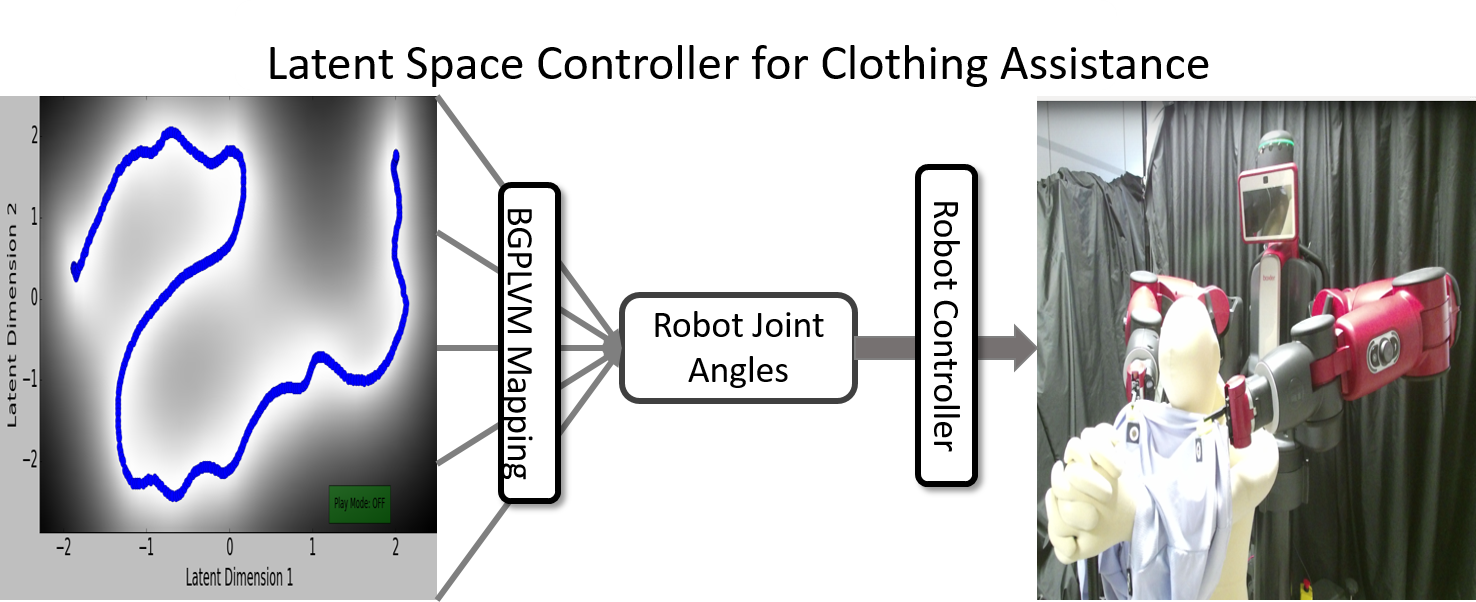
\includegraphics[width=0.5\textwidth]{controller.png}
  \caption{Overview of latent space controller for performing clothing tasks.}
  \label{figure:realtime}
\end{figure}

Motor skills for clothing assistance lie in an high dimensional kinematic space given by joint angle trajectories of a 7 DOF dual-arm robot. The robot also has to maintain several task space constraints such as the coupling with a clothing article along with operating safely in close proximity to a human subject as shown in Figure~\ref{figure:setup}. These task space constraints are difficult to be modeled in the kinematic space as they are non-linearly related to each other. To address these problems, we propose the use of BGPLVM for learning a latent space that efficiently encodes clothing assistance skills. BGPLVM results in the learning of a low-dimensional latent space through a nonlinear and data-efficient mapping to the kinematic space. Furthermore, we train the model using successful trajectories of the robot performing clothing tasks so that the resultant latent space generates robot trajectories that follow task space constraints. The Bayesian treatment avoids over fitting to the training data and automatic inference of the latent space dimensionality through the use of ARD kernel.

In this study, we consider the clothing task where a dual-arm robot clothes a soft mannequin with a T-shirt which is initially resting on the mannequin's arms. The purpose of the BGPLVM model is to learn a latent representation $\mathbf{X} = [\mathbf{X}_1, \cdots, \mathbf{X}_N]$ from a dataset of 7-DOF dual-arm robot poses $\mathbf{Y} = [\mathbf{y}_1, \cdots, \mathbf{y}_N]$. We represent the robot poses in two alternate ways i.e. 1) Kinematic representation given by joint angles of both 7-DOF arms $D_K = 14$ and 2) Task space representation given by the end-effector pose of both robot arms which comprises the Cartesian position ${P_X,P_Y,P_Z} \in \mathbb{R}^3$ and orientation represented using a quaternion ${O_X,O_Y,O_Z,O_{\omega}} \in \mathbb{R}^4$ forming a 14-dimensional space $D_T = 14$. The dataset $\mathbf{Y}$ was obtained from a collection of successful clothing assistance demonstrations performed by the robot for various postures of the mannequin. We set the dimension of the latent space as $q = 5$, however the dimensionality is eventually inferred through the training of the ARD kernel weights as explained in Section~\ref{section:bgplvm}.

\subsection{Latent Space Robot Controller}
\label{section:controller}

There can be several types of failure scenarios when the robot performs clothing tasks. While clothing, the T-shirt collar could get stuck on the mannequin's head and while unclothing, the T-shirt could get stuck in the mannequin's shoulder joints. To recover from these failures, not only is the trajectory of the robot important, but also the speed of execution. Imparting these skills through kinesthetic movement of the arms can be difficult for a bulky robot and could lead to noisy demonstrations. To address this problem, we have implemented a real-time controller that gets an input signal from the BGPLVM latent space. The BGPLVM model learns a mapping from the low dimensional latent space to the robot kinematic space such that a trajectory of latent points generates a trajectory on the dual-arm robot. This interface can be used as a tool for Learning from Demonstration (LfD) wherein, the necessary clothing skills are imparted to the robot by using cursor control over the latent space as shown in Figure~\ref{figure:realtime}.

\section{Results}
\label{section:results}

In this section, we present the results of using BGPLVM as a representation for clothing assistance motor skills. The experimental setup includes the Baxter 7 DOF dual-arm robot performing clothing tasks and a soft mannequin as the subject as shown in Figure~\ref{figure:setup}. The clothing task is to cloth the mannequin with a T-shirt which is initially resting on the mannequin's arms. The evaluation is presented in two parts: Section~\ref{section:performance} demonstrates the generalization capability of BGPLVM to unseen environmental settings and Section~\ref{section:controllerres} presents the performance of the real-time controller presented in Section~\ref{section:controller}.

\subsection{Predictive Performance}
\label{section:performance}

\begin{figure}[t]
  \centering
  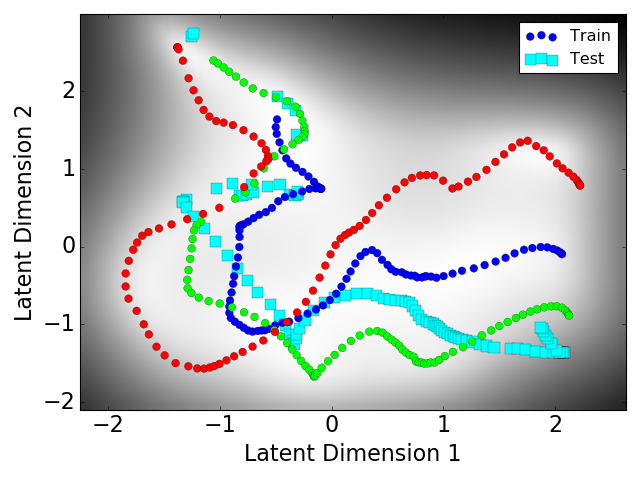
\includegraphics[width=0.5\textwidth]{latentspace.png}
  \caption{Latent Space of BGPLVM trained on Joint Angle dataset of clothing tasks. Latent points include 3 train trials and 1 test trial.}
  \label{figure:latent}
\end{figure}

In this experiment, the generalization capability of BGPLVM for performing clothing tasks is evaluated. The evaluation dataset contains 4 clothing trials that were obtained for 4 different postures of the mannequin wherein the elevation of the arms were varied forming different angles $\{65^o, 70^o, 75^o, 80^o\}$ with the mannequin's body. The clothing trial for $75^o$ was left out as the test data and BGPLVM models were trained for the remaining 3 clothing trials. Trained models for both the joint angles (JA) and end-effector Cartesian positions (EE) resulted in 2 dimensional latent spaces. The resultant latent space for the JA model is visualized in Figure~\ref{figure:latent}. It can be seen that smooth latent trajectories are formed for each clothing trial capturing the dynamics of performing the task. Furthermore, a smooth latent trajectory exists for the test clothing trial as well indicating the possibility for a reinforcement learning framework to generalize to the new posture.

\subsection{Controller Demonstration}
\label{section:controllerres}

In this section, the latent space controller presented in Section~\ref{section:controller} is demonstrated. The latent space for the controller is trained for the joint angles of a clothing trial obtained from kinesthetic demonstration by a human. The resultant model represented the data in a 2 dimensional latent space. Cursor control on the latent space was able to reproduce the clothing demonstration even when the latent trajectory was different from the training latent points as shown in Figure~\ref{figure:controller}. The resultant latent dimensions further captured a specific aspect of the clothing motor-skills. For example, the most significant dimension captured the horizontal motion of the arms along the mannequin while maintaining the constraints for clothing. The second dimension captured various vertical motions of pulling up the T-shirt in the beginning and pulling it down along the torso at the end.

\section{Conclusion}
\label{section:conclusion}

Motor-skills learning for robotic clothing assistance task involves a high dimensional kinematic search space and maintaining several task space constraints. In this study, we have presented the use of Bayesian Gaussian Process Latent Variable Model (BGPLVM) as a representation for encoding motor-skills to perform clothing assistance task. The experimental results indicate our method as a promising approach in combination with reinforcement learning. A latent space representation can be learned from multiple observation spaces using Manifold Relevance Determination (MRD)~\cite{mrd} which is an extension of BGPLVM. Based on this flexibility, our future work will be to learn models that explicitly incorporates visual information of the relationship between the human and cloth. The long term goal will be to develop a policy search reinforcement learning framework that relies on the use of BGPLVM.

\begin{figure}[t]
  \centering
  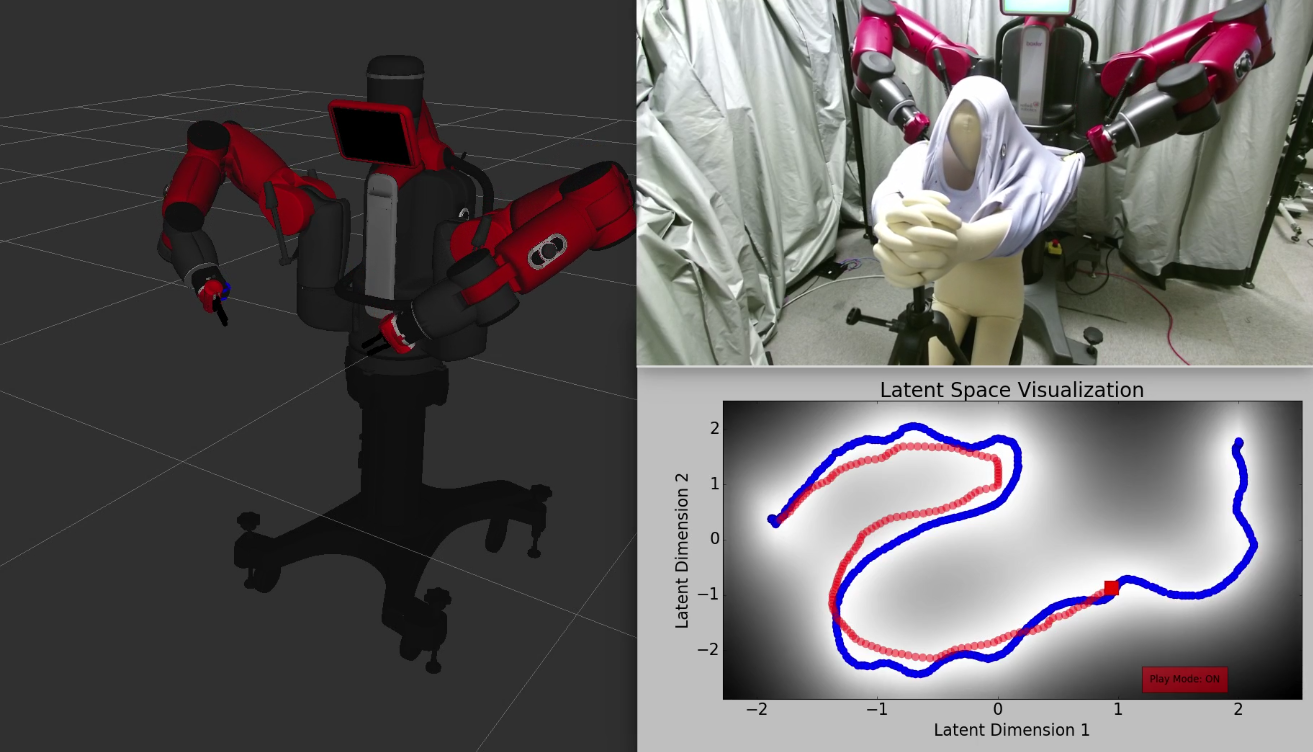
\includegraphics[width=0.5\textwidth]{controller2.png}
  \caption{Cursor control on BGPLVM latent space to perform clothing task. Figure on left shows simulation of robot pose, right top shows robot performing clothing task and right bottom shows cursor control in latent space.}
  \label{figure:controller}
\end{figure}

\section*{Acknowledgement}
This work was supported in part by ImPACT Program of Council for Science, Technology and Innovation (Cabinet Office, Government of Japan) 2015-PM07-36-01. This work was also supported in part by the Grant-in-Aid for Scientific Research from Japan Society for the Promotion of Science (No. 16H01749).

\small

\begin{thebibliography}{15}
\bibitem{yamazaki}
K. Yamazaki, R. Oya, K. Nagahama, K. Okada, and M. Inaba, ``Bottom dressing by a life-sized humanoid robot provided failure detection and recovery functions'' in Proc. of the IEEE Intl. Conf. on System Integration (SII), 2014.

\bibitem{gao}
Y. Gao, H. J. Chang, and Y. Demiris, ``User modelling for personalised dressing assistance by humanoid robots'' in Proc of the IEEE Intl. Conf. on Intelligent Robots and Systems (IROS), 2015.

\bibitem{tamei}
T. Tamei, T. Matsubara, A. Rai, and T. Shibata, ``Reinforcement Learning of Clothing Assistance with a Dual-arm Robot'' in Proc. of the IEEE-RAS Intl. Conf. on Humanoid Robots (Humanoids), 2011.

\bibitem{bgplvm}
Titsias, M. K., and Lawrence, N. D, ``Bayesian Gaussian process latent variable model'' in Proc. of the Intl. Conf. on Artificial Intelligence and Statistics, 2010.

\bibitem{bitzer}
Bitzer, S., Howard, M., and Vijayakumar, S, ``Using dimensionality reduction to exploit constraints in reinforcement learning'' in Proc. of the IEEE Intl. Conf. on Intelligent Robots and Systems (IROS), 2010.

\bibitem{luck}
Luck, K. S., Neumann, G., Berger, E., Peters, J., and Ben Amor, H, ``Latent space policy search for robotics'' in Proc. of the IEEE Intl. Conf. on Intelligent Robots and Systems (IROS), 2014.

\bibitem{mrd}
Damianou, A., Ek, C., Titsias, M., and Lawrence, N, ``Manifold relevance determination'' in Proc. of the Intl. Conf. on Machine Learning, 2012.

\end{thebibliography}

\end{document}
